\chapter{Results: statistical data and webGIS interface}

    \vspace{0.06\textheight}
    \begin{chaptersum}
        \blindtext[2]
    \end{chaptersum}

    To ensure the correctness of the proposed methods, all the results obtained will be compared to the most up to date informations published by dott.ssa Angela Laterza in 2013 \cite{laterza}. Most of the comparisons show a good correspondence among datasets; this result is more impressive when related with the time employed to automatically generate the data, which in most cases is at least one order of magnitude less than the manual method. The last section of this chapter presents one of the fundamental components of the proposed system, the web interface, which connects all the functions, methods and algorithms previously described with an interface conceived to be clear and simple for the end user.

    \section{Statistical results}
        \subsection{Ditches and compounds classification}
            The method described in \fref{sec:distinguish} has enabled the operator to write once all the attributes in every ditch and compound, distinguishing them. The procedure requires around \SI{1}{\minute} for each settlements, compared to nearly \SI{1}{\hour} in a non-automatized approach (depending on the number of geometries in the settlement). The whole set of 11 settlements containing 199 geometries has been analyzed in around \SI{10}{\minute}. The plots in \fref{fig:graph-num-compound} and \fref{fig:graph-num-ditch} compare the number of compounds and ditches distinguished as such from the human brain-eye system --- as reported in \cite{laterza} --- and the values calculated in the current work, showing a perfect matching between the two datasets. The settlements are described using their site code (see \fref{tab:layers}).

            \begin{figure}[H]
                \centering
                \begin{tikzpicture}
                    \pgfplotstableread{tab/raw/number-comp}{\loadedtable}
\small

\begin{axis}[
    width=1\textwidth,
    height=0.5\textwidth,
    ybar,
    ymin=0,
    enlarge x limits,
    xlabel=settlements,
    xlabel shift=-5pt,
    ylabel=compounds $(n)$,
    xtick={1,...,11},   % indicates xticks going from 1 to 11
    xticklabels from table={\loadedtable}{set},
    xticklabel style={rotate=45,font=\scriptsize},
    xticklabel shift=-3pt,
    legend style={font=\scriptsize,draw=black!40}
]
    \addplot table[x=id, y=laterza] from \loadedtable;
    \addplot table[x=id, y=current] from \loadedtable;
    \legend{Lat13,current}
\end{axis}

                \end{tikzpicture}
                \caption[The number of compounds in \cite{laterza} compared to the results of the proposed method.]{The number of compounds automatically calculated for all the analyzed settlements, compared with the results reported in \cite{laterza}.}
                \label{fig:graph-num-compound}
            \end{figure}

            \begin{figure}[H]
                \centering
                \begin{tikzpicture}
                    \pgfplotstableread{tab/raw/number-ditch}{\loadedtable}
\small

\begin{axis}[
    width=1\textwidth,
    height=0.5\textwidth,
    ybar,
    ymin=0,
    enlarge x limits,
    xlabel=settlements,
    xlabel shift=-5pt,
    ylabel=ditches,
    xtick={1,...,11},   % indicates xticks going from 1 to 11
    xticklabels from table={\loadedtable}{set},
    xticklabel style={rotate=45,font=\scriptsize},
    xticklabel shift=-3pt,
    legend style={font=\footnotesize,draw=black!40}
]
    \addplot table[x=id, y=laterza] from \loadedtable;
    \addplot table[x=id, y=current] from \loadedtable;
    \legend{Laterza 2013,current}
\end{axis}

                \end{tikzpicture}
                \caption[The number of ditches in \cite{laterza} compared to the results of the proposed method.]{The number of ditches automatically calculated for all the analyzed settlements, compared with the results reported in \cite{laterza}.}
                \label{fig:graph-num-ditch}
            \end{figure}

            Having all the statistics registered in a database, is very easy to extract further data; the \fref{fig:graph-perim-class}, for example, shows the frequency of perimeter's classes for all the compounds; it si evident that most of the analyzed compounds are contained in the first class of perimeters, ranging from \SI{96.6}{\meter} to \SI{103}{\meter}.

            \begin{SCfigure}
                \caption[Frequency of all the analyzed compounds for each perimeter class, with $k=5$.]{Frequency of all the analyzed compounds for each perimeter class, with the default number of classes $k=5$. Class $6$ has been removed since only ditches belong to it.}
                \begin{tikzpicture}
                    \pgfplotstableread[col sep=comma]{tab/raw/perim-class.csv}{\loadedtable}
\small

\begin{axis}[
    width=0.5\textwidth,
    height=0.5\textwidth,
    ybar,
    ymin=0,
    enlarge x limits,
    xlabel=perimeter classes,
    xlabel shift=-5pt,
    ylabel=frequency $(n)$,
    xtick={1,...,5},   % indicates xticks going from 1 to 11
    xticklabels from table={\loadedtable}{class},
    xticklabel style={font=\scriptsize},
    xticklabel shift=3pt
]
    \addplot table[x=id, y=freq] from \loadedtable;
\end{axis}

                \end{tikzpicture}
                \label{fig:graph-perim-class}
            \end{SCfigure}

        \subsection{Derived areas}
            % min, max, avg area

            The method described in \fref{sec:comp-area} has produced the results shown in the rightmost column of \fref{fig:graph-area} for each analyzed settlement. The results obtained in few minutes with the automated method are accurate enough to be closely compared with ones drawn by hand using GIS tools from the operator during several days of work, as published in \cite{laterza}.
            As will be reported in the next section, the \emph{Salerno 13} settlement shows a small discordance with the previously published data (although not conspicuous).

            \begin{figure}[H]
                \centering
                \begin{tikzpicture}
                    \pgfplotstableread[col sep=comma]{tab/raw/aree.csv}{\loadedtable}
\small

\begin{axis}[
    width=1\textwidth,
    height=0.5\textwidth,
    ybar,
    ymin=0,
    enlarge x limits,
    xlabel=settlements,
    xlabel shift=-5pt,
    ylabel=area $(\si{\meter\squared})$,
    xtick={1,...,11},   % indicates xticks going from 1 to 11
    xticklabels from table={\loadedtable}{set},
    xticklabel style={rotate=45,font=\scriptsize},
    xticklabel shift=-3pt,
    legend style={font=\footnotesize,draw=black!40}
]
    \addplot table[x=id, y=laterza] from \loadedtable;
    \addplot table[x=id, y=current] from \loadedtable;
    \legend{Laterza 2013,current}
\end{axis}

                \end{tikzpicture}
                \caption[Areas of all the analyzed settlements compared with ones published in \cite{laterza}.]{Areas of all the analyzed settlements, compared to ones defined in \cite{laterza}. The proposed values fit well with published data.}
                \label{fig:graph-area}
            \end{figure}

        \subsection{Derived perimeters}
            % mix, max, avg perimeter
            
            As explained in \fref{sec:comp-area}, the perimeter for each compound is directly derived from the geometry of its area, to reproduce the results obtained in \cite{laterza}. The error seen in the previous section for the \emph{Salerno 13} settlement has repercussions on the perimeter. This behavior can be attributed to an error in the area derivation using the automated method: this prevented the construction of the area geometry for 8 compounds (out of 36, for that settlement), modifying the total area value for the settlement (and the relative derived perimeter). This is the only known error in the proposed method.

            \begin{figure}[H]
                \centering
                \begin{tikzpicture}
                    \pgfplotstableread[col sep=comma]{tab/raw/perim.csv}{\loadedtable}
\small

\begin{axis}[
    width=1\textwidth,
    height=0.7\textwidth,
    ybar,
    ymin=0,
    enlarge x limits,
    xlabel=settlements,
    xlabel shift=-5pt,
    ylabel=perimeter $(m)$,
    xtick={1,...,11},   % indicates xticks going from 1 to 11
    xticklabels from table={\loadedtable}{set},
    xticklabel style={rotate=45,font=\scriptsize},
    xticklabel shift=-3pt,
    legend style={font=\footnotesize,draw=black!40}
]
    \addplot table[x=id, y=laterza] from \loadedtable;
    \addplot table[x=id, y=current] from \loadedtable;
    \legend{Laterza 2013,current}
\end{axis}

                \end{tikzpicture}
                \caption[Comparison of published perimeters with ones obtained with the proposed method.]{Comparison of the total perimeters obtained for all the compounds in each analyzed settlement with the values published in \cite{laterza}, showing a good correspondence.}
                \label{fig:graph-perim}
            \end{figure}

            Minor dissimilarities with some settlements (\emph{Anglisano 2}, \emph{Lore 2}) depend on the nature of the derivation method itself: in respect to the flaws listed in \fref{sec:gis-data-management}, the difference between geometries traced by hand (subject to magnification errors) and computed using the algorithm is amplified when single differences are summed up to produce data referred to the whole settlement.

            % statistical difference between perimeters of single compounds in one settlement (anglisano?)

        \subsection{Orientation discovering}
            % min, max, avg access length
            % is there any relation between orientation and access length?

            Automating the discovering of the compounds' orientations has been the hardest task, since involves the derivation of multiple geometries for each compound (see \fref{sec:orientation}).
            The information about compounds' orientation for 155 compounds in all the analyzed sites has been automatically calculated and required less than \SI{4}{\minute} to generate and save the relevant data to the database, while manually defining an orientation index as for a ``normal'' approach requires several days of work.
            
            The results plotted in \fref{fig:graph-orient} show that the general trend in the orientations calculated in this work is very similar to the one published in \cite{laterza}. However, the significance of this calculation can be improved, since presenting each orientation as an interval of values (e.g.\ NE contains all the values ranging from \SI{0}{\degree} to \SI{45}{\degree}) is an operation of classification itself, and has caused a loss of detail. This has been done to register values comparable to the ones defined in \cite{laterza}. At the current status, nothing can be done to prove which measurement is nearest to reality, but the assumption that both datasets share the same trends seems a result good enough to state that the automated method is fully functional.

            \begin{figure}[H]
                \centering
                \begin{tikzpicture}
                    \pgfplotstableread[col sep=comma]{tab/raw/orient.csv}{\loadedtable}
\small

\begin{axis}[
    width=1\textwidth,
    height=0.5\textwidth,
    ybar,
    ymin=0,
    enlarge x limits,
    xlabel=orientation,
    xlabel shift=-5pt,
    ylabel=frequency,
    xtick={1,...,8},   % indicates xticks going from 1 to 11
    xticklabels from table={\loadedtable}{orient},
    xticklabel style={rotate=45,font=\scriptsize},
    xticklabel shift=-3pt,
    legend style={font=\footnotesize,legend pos=north west,draw=black!40}
]
    \addplot table[x=id, y=laterza] from \loadedtable;
    \addplot table[x=id, y=current] from \loadedtable;
    \legend{Laterza 2013,current}
\end{axis}

                \end{tikzpicture}
                \caption[Orientation of compounds for all the settlements calculated in this work compared with know data.]{Compounds' orientation calculated using automated algorithm compared to manually derived data.}
                \label{fig:graph-orient}
            \end{figure}

            Before the work of dott.ssa Laterza in 2013, the only available data about the compounds' orientation of the Tavoliere settlements were in \textcite[appx.~IV]{jones-tavoliere}, reported as data tables and derived drawing by hand on graph paper, on top of aerial photos. The orientation data contained in the tables refers to the ``average orientation'' of compounds in some settlements, and have not been calculated for each compound. Thus, comparing these general values to \emph{atomized} data obtained from calculation on every single compound as done so far in this work, may appear risky from the scientific point of view. Nonetheless, a graphical comparison may still be useful to visually find some trends --- if any. 

            \cite{jones-tavoliere} reports orientation data of 24 settlements, and just few of these are referable to the set analyzed in this work. Thus, orientation data from all the sources (\cite{laterza}, \cite{jones-tavoliere} and this work) have been calculated as percentage referred to the total analyzed compounds. Results are shown in \fref{fig:graph-orient-jones}.

            \begin{figure}[H]
                \centering
                \begin{tikzpicture}
                    \pgfplotstableread[col sep=comma]{tab/raw/orient-jones.csv}{\loadedtable}
\small

\begin{axis}[
    width=1\textwidth,
    height=0.5\textwidth,
    bar width=7pt,
    ybar,
    ymin=0,
    enlarge x limits,
    xlabel=orientation,
    xlabel shift=-5pt,
    ylabel=percentage $(\%)$,
    xtick={1,...,8},   % indicates xticks going from 1 to 8
    xticklabels from table={\loadedtable}{orient},
    xticklabel style={rotate=45,font=\scriptsize},
    xticklabel shift=-3pt,
    legend style={font=\scriptsize,legend pos=north west,draw=black!40}
]
    \addplot table[x=id, y=laterza] from \loadedtable;
    \addplot table[x=id, y=current] from \loadedtable;
    \addplot table[x=id, y=jones] from \loadedtable;
    \legend{Lat13,current,JST87}
\end{axis}

                \end{tikzpicture}
                \caption[Comparison of automatically derived orientation data with the other sources.]{Comparison of the orientation data, from left: manually derived by \citeauthor{laterza}, automatically calculated in the current work and derived by hand by \citeauthor{jones-tavoliere} in 1987. The latter refers to average settlements' orientation, while the others to average compounds' orientation.}
                \label{fig:graph-orient-jones}
            \end{figure}

        \subsection{The web interface structure\label{sec:webgis}}
            Having defined all the algorithms to derive geometries and data from the input vectors, the next step concerned a way to make these tool accessible to the operator, even ones with less experience. To ease the development of a standard compliant interface the Django \emph{framework} has been used; both the framework and the algorithms share the same open source programming language, Python.
            Django enables the development of web-based products; thus, the whole set of statistical tools described in this work are accessible as a web service, simply connecting to the web address using a normal web browser.

            Very little effort is required to start with calculations on a settlement. The web interface is password protected, thus each operator have to access with his own credentials. After, the user just have to open an ESRI Shapefile containing vector data of a single settlement in a GIS software suite, and clean it from all the geometries but those representing ditches and compounds. To ease the upload, the operator have to enclose the abovementioned Shapefile in a compressed archive (\emph{.zip} is the preferred format). This process guarantees a fast upload using the web interface shown in \fref{fig:shp-upload}.
            
            The developed web interface consists of few pages; briefly listed:

            \begin{description}
                \item[Shapefiles list] the start page, lists all the uploaded Shapefiles and has a button redirecting to the upload page; if no Shapefile has been uploaded, the list is empty (\fref{fig:shp-list});
                \item[upload page] enables the user to upload a new Shapefile, which is consequently saved to the software's internal database (\fref{fig:shp-upload});
                \item[Shapefile details] the most relevant page, shows a map of the selected Shapefile on the left and a list of all possible statistics on the right (\fref{fig:shp-details}); every statistic has its own button, which starts the calculation when clicked; if a statistic has been calculated, the relevant row has a green background, or red on the contrary; the upper right part of the page contains buttons to manage the current Shapefile, enabling the deletion, statistics plotting or downloading.
                \item[Jenks classification] while all other algorithms do not need any interaction with the user, the Jenks Natural Breaks classification sometimes needs the number of classes $k$ to be redefined by the operator; for this purpose a wizard has been created (\fref{fig:shp-wizard}); it is launched pressing the button associated with the row containing the number of ditches or compounds in the Shapefile details page; the user can change the $k$ value and the colored map representing classified values is refreshed on the fly.
            \end{description}

            \pagebreak

            \vfill

            \begin{figure}[H]
                \caption[Screenshots of the main tools of the software created to automate statistical calculations.]{Main tools included in the software used to automate statistical calculations of the data presented in this work. The calculation functions are accessible from buttons on the interface. All the images show example calculations operated on the \emph{Anglisano 1} settlement.}
                \label{fig:screenshots}
            \end{figure}

            \vfill

            \begin{figure}[H]
                \ContinuedFloat
                \begin{subfigure}[b]{1\textwidth}
                    \centering
                    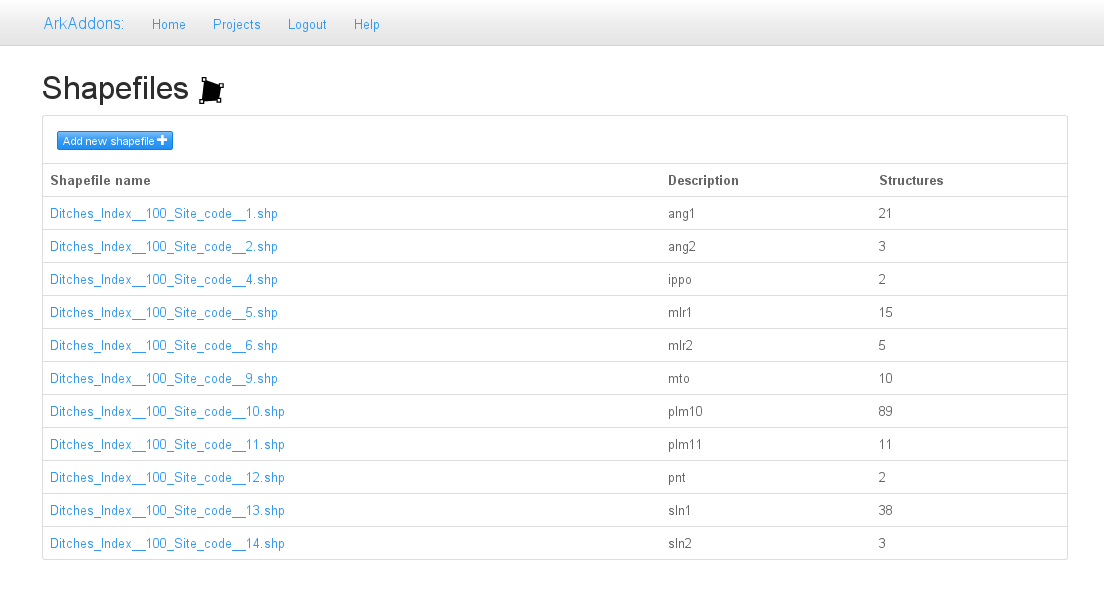
\includegraphics[width=1\textwidth]{img/shp-list}
                    \caption{The start page lists all the uploaded ESRI Shapefiles, one for each settlement; the button on the upper left redirects to the upload file page. The rightmost column of the list shows an automatically generated sum of all the geometries contained in the loaded Shapefiles.}
                    \label{fig:shp-list}
                \end{subfigure}
            \end{figure}

            \vfill

            \begin{figure}[H]
                \ContinuedFloat
                \begin{subfigure}[b]{1\textwidth}
                    \centering
                    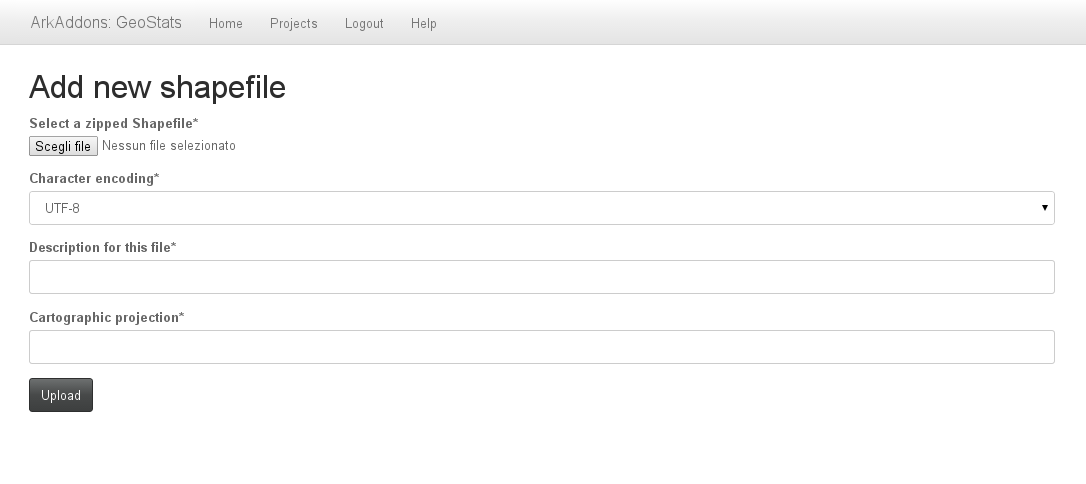
\includegraphics[width=1\textwidth]{img/shp-upload}
                    \caption{Using the upload page, the user can upload a new settlement's ESRI Shapefile; a description, character encoding and cartographic projection for the file can be specified; when the loading is completed, all the geometries are saved in an internal database.}
                    \label{fig:shp-upload}
                \end{subfigure}

            \end{figure}

            \pagebreak

            \vfill

            \begin{figure}[H]
                \ContinuedFloat
                \begin{subfigure}[b]{1\textwidth}
                    \centering
                    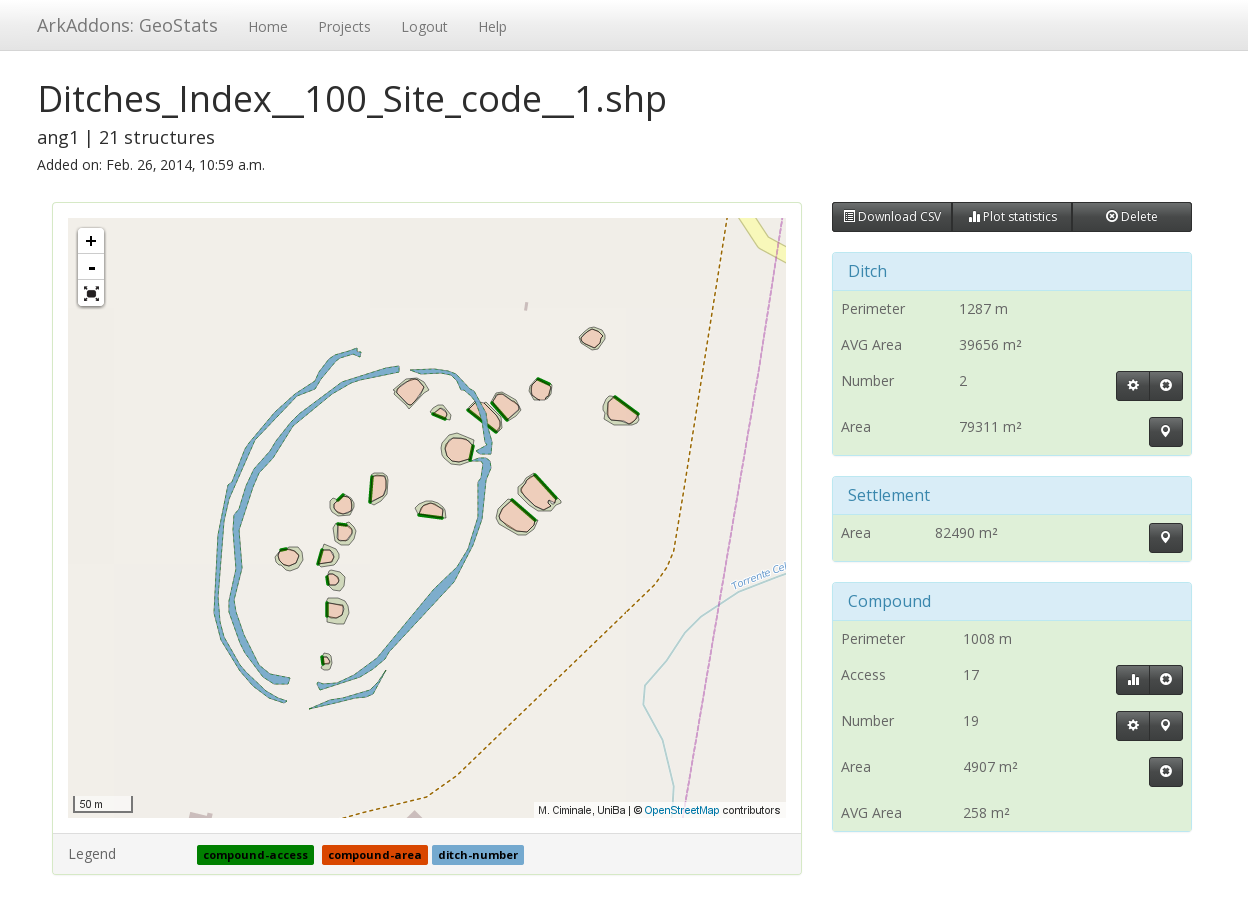
\includegraphics[width=0.95\textwidth]{img/shp-details}
                    \caption{Shapefile details page; the map shows the base layer and some more layers with data automatically derived from statistical calculations; the respective values for the statistics are shown in the table on the right.}
                    \label{fig:shp-details}
                \end{subfigure}
            \end{figure}

            \vfill

            \begin{figure}[H]
                \ContinuedFloat
                \begin{subfigure}[b]{1\textwidth}
                    \centering
                    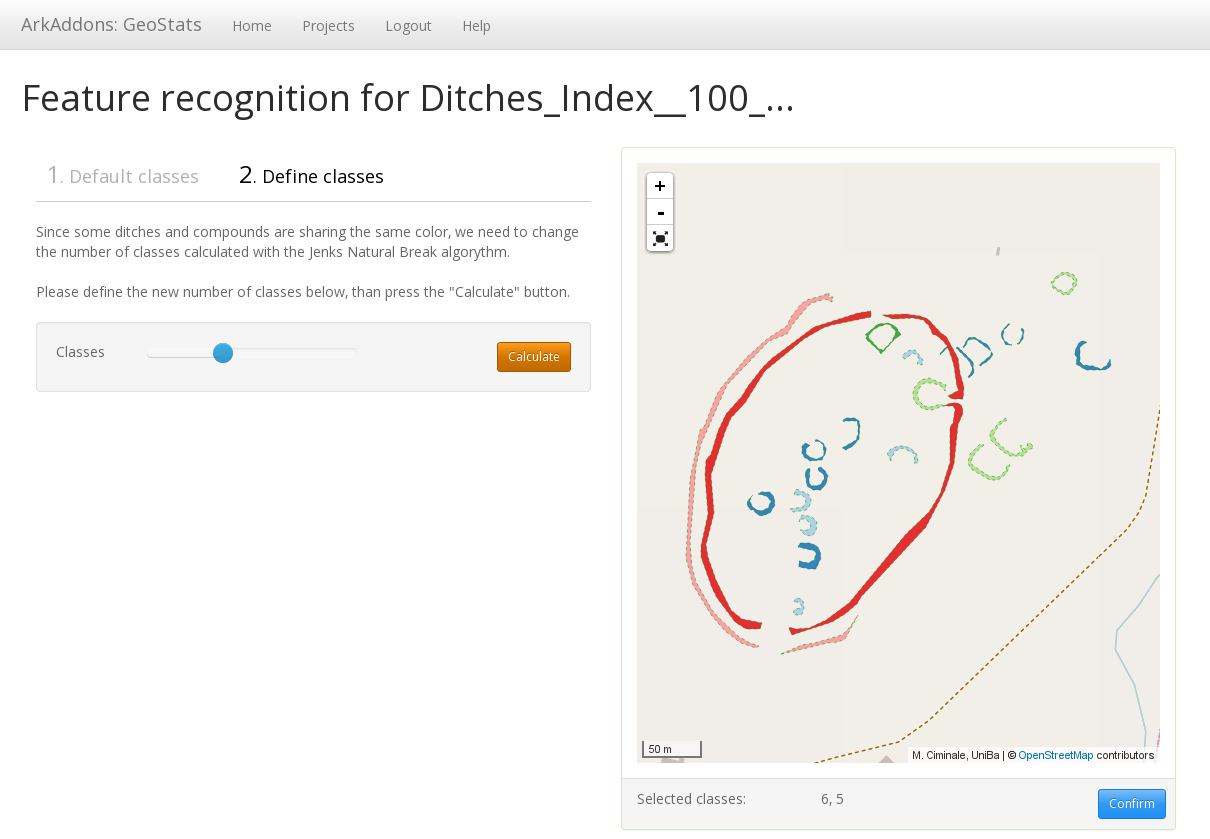
\includegraphics[width=0.95\textwidth]{img/shp-wizard}
                    \caption{The wizard used to show compounds geometries classified using the Jenks Natural Breaks, with slider to redefine the number of $k$ classes to find the best fit with perimeters.}
                    \label{fig:shp-wizard}
                \end{subfigure}
            \end{figure}

            \vfill

        \section{Achieved results}
            % automated time consuming operations
            % avoided magnification errors, improved precision
            % boosted reproducibility
            % standard format data export -- csv
            % pleasant interface

        \section{Software technical specifications}
            From the technical point of view, the software has been implemented using the Django framework, version 1.6 and the relative geographic extension (\emph{GeoDjango}); this offers a granular user access control system, and powerful tools to write object-oriented code to manage the single Shapefiles during calculations. The most important parts of the presented algorithms have been realized using the GEOS components of the GeoDjango extension.

            The webGIS interface has been built using the LeafletJS JavaScript library, which receives geoJSON formatted outputs from Django when a layer is called pressing the relative button. All the graphical components are provided by the Twitter Bootstrap tools collection, boosting the usability of the website.
            
            The software relies on the SpatiaLite geographical database to register, manage and do some queries with the processed data; it has been chosen since it is a full-featured, self-contained database, very easily manageable when working with Python, since it is included in all the standard GNU/Linux repositories and does not require any particular configuration or setup; moreover, it can also be shipped as a normal file when distributing the software.

            \subsection{Scientific reproducibility: the open source approach advantage}
                % only open source software
                % free software definition
                % best control of calculation processes
                % open to contribution from scientific community
                % low cost

